%
% GNU, Yi Zhang, 2018
%

\section{多种群协同进化}\renewcommand{\baselinestretch}{1.5} \normalsize:

\frame{ \frametitle{定义}
	\setlength{\parindent}{2em}
	协同演化算法(coevolutionary algorithm,CEA)通过构造两个或多个种群,
	建立它们之间的竞争或合作关系,多个种群通过相互作用来提高各自性能,
	适应复杂系统的动态演化环境, 以达到种群优化的目的.
}

\frame{ \frametitle{背景}
	\setlength{\parindent}{2em}
	演化算法,基于个体自身适应度:\\
	~~1.~未成熟收敛\\
	~~2.~收敛速度慢\\
	~\\
	~\\
	协同演化算法,一个个体适应度在与其他个体(同种群个体,不同种群个体)的交互过程中计算.
}

\frame{\frametitle{framework}
	\begin{figure}[ht]
		\centering	
		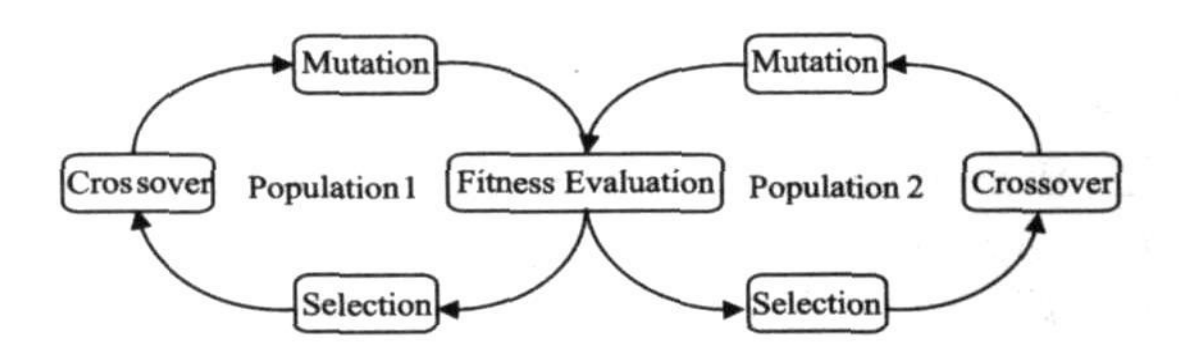
\includegraphics[scale=0.25]{../images/cc_framework.png}
		\caption{the framework of CEA}
		\label{fig:label}
	\end{figure}
}

\frame{ \frametitle{应用}
	\setlength{\parindent}{5em}
	1> ~~  函数优化\\
	2> ~~  多目标优化\\
	3> ~~  分类\\
	4> ~~  图像分割\\
	5> ~~  神经网络设计\\
	6> ~~  工程设计
}

\frame{ \frametitle{ 分类 }
	\setlength{\parindent}{4em}
	>> ~~  合作型协同进化算法(Coop-CEA)\\
	~\\
	~\\
	>> ~~  竞争型协同进化算法(Comp-CEA)\\
}

%合作型协同进化算法
\frame{ \frametitle{ Coop-CEA }
	\setlength{\parindent}{2em}
	Coop-CEA使用分治策略将演化算法(EA)应用于大型复杂问题的中.
	原始问题被分解成更小的模块,并且每个模块都被分配到一个物种。
	这些物种大多分开进化,唯一的合作发生在适应性评估期间。
}


\frame{ \frametitle{ Coop-CEA一般框架 }
	\begin{itemize}
		\item<1->  Decompose an objective vector into m low-dimensional subcomponents.
		\item<2->  Set i = 1 to start a new cycle.
		\item<3->  Optimize the ith subcomponent with a certain EA for a predefined number of fitness evaluations (FEs).
		\item<4->  If i < m then i ++, and go to Step 3.
		\item<5->  Stop if halting criteria are satisfied; otherwise go to Step 2 for the next cycle.
	\end{itemize}
}

\frame{ \frametitle{ Coop-CEA任务分解 }
	\setlength{\parindent}{2em}
	Coop-CEA中,每个个体只表示解的一部分,每个种群求一个部分解.把多个自种群的最终解连接起来就是Coop-CEA的解.\\
	~\\
	任务分解:\\
	1.~随机分解:随机选择基因的顺序\\
	2.~扰动:使用扰动决策变量尝试对变量进行分组\\
	3.~模型构建:基于个体数量的概率模型
}

\frame{ \frametitle{ Coop-CEA适应度计算 }
	\setlength{\parindent}{2em}
	Coop-CEA中,个体的适应度表现为与其他各种群的合作能力\\
	从其它的每一个子群体接收若干“合作者”来同该个体合作,一起组成若干完整的解。求得的适应度中的最佳值作为所求个体的适应度。\\
	~\\
	合作者可以随机选择,也可以选择种群中最佳个体\\
	合作者可多可少
}

%竞争型协同进化算法
\frame{ \frametitle{ Comp-CEA }
	\setlength{\parindent}{2em}
	竞争型协同进化的核心思想就是物种间的相互作用,这种相互作用的结果使得物种获得进化的动力\\
	~\\
	一个种群中的个体适应度是由其他种群的个体的一系列竞争作用来决定的协同进化
}

\frame{ \frametitle{ Comp-CEA workfow }
	\setlength{\parindent}{2em}
	BEGIN\\
	~Initialize Pop1, Pop2\\
	~Let Pop1 serve as learner\\
	~Select the set of evaluators(E) from Pop2\\
	WHILE( not termination )\\
	~~~~Evaluation(learner)\\
	~~~~Selection(learner)\\
	~~~~Crossover(learner)\\
	~~~~Mutation(learner)\\
	~~~~Interehange the individuals in Pop1 and Pop2\\
	~~~~Select the set of evaluators form Pop2\\
	END
}

\frame{ \frametitle{ Comp-CEA适应度计算 }
	\setlength{\parindent}{2em}
	竞争适应度:一个种群的个体对对手竞争力的大小\\
	~\\
	~\\
	种群适应度:一个种群相对其他种群的竞争力的大小
}

\frame{ \frametitle{ Comp-CEA适应度计算 }
	\setlength{\parindent}{2em}
	简单竞争适应度\\
	\begin{equation}
		\forall i \in L \Rightarrow CF_i = \sum_{j \in E,\;i\;defeat\;j}1
	\end{equation}\\
	共享竞争适应度\\
	\begin{equation}
		\forall j \in E \Rightarrow N_j = \sum_{k \in L,\;k\;defeat\;j}1
	\end{equation}
	\begin{equation}
		\forall i \in L \Rightarrow CF_i = \sum_{j \in E,\;i\;defeat\;j}\frac{1}{N_j}
	\end{equation}\\
	~\\
	L:学习者~~~~~E:评价者
	
}

\frame{ \frametitle{ Comp-CEA评价者选取 }
	\setlength{\parindent}{2em}
	具有相同染色体的个体,可能由于临时对手的不同,得到不同的适应度\\
	~\\
	~~~随机配对\\
	~~~随机选定多个临时对手\\
	~~~穷举
}

%end